Talvez o melhor modo de iniciar o assunto seja tratar de uma de suas aplicações, uma vez que a contextualização ajuda a trazer um conceito bem abstrato para o nosso mundo real.

Certamente você já viu uma figura com muitas palavras e cada uma delas com tamanho de fonte diferente. Essa é a representação gráfica do que é conhecido tecnicamente como "bag of words", ou \textbf{saco de palavras}, em tradução livre.

\begin{figure}[h]
\centering
\caption{Exemplo de bag of words}
\vspace{0.25cm}
\label{fig:bag}
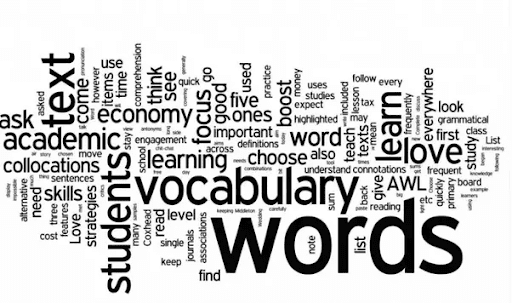
\includegraphics[width=0.9\linewidth]{imagens/bag.png}
%\caption*{Fonte: http://www.verbatimmag.com/WordWords.html}
\end{figure}

A construção desta imagem envolve uma lista de palavras (óbvio) obtidas de alguma fonte e a operação de cálculo da frequência de cada palavra, ou seja, quantas vezes a dada palavra aparece em uma lista. A palavra com maior frequência aparece mais em fonte maior na imagem.

Aqui aparece nosso primeiro problema: \textbf{como obter essa frequência de modo rápido}? Ou ainda de modo mais específico: \textbf{como armazenar essa frequência}? Existem diversas soluções para esse problema, certo?

Para deixar. momentaneamente, tudo mais claro e fácil, no lugar de palavras usaremos uma chave única para cada uma dessas palavras e temos mais um problema: \textbf{como gerar essas chaves}? Seria algo como "bolo" e sua chave gerada pelo algoritmo \textbf{SHA 256}. Quer testar? Os comandos mostrados a seguir ilustram o retorno do algoritmo que calcula o hash\footnote{Calma... chegaremos rapidamente ao conceito.} da palavra "Uniara".

\begin{tcolorbox}[title=No sistema operacional Windows]
    echo "Uniara" $|$ CertUtil -hashfile - SHA256
\end{tcolorbox}

\begin{tcolorbox}[title=No sistema operacional Linux ou MacOS]
    echo -n "Uniara" $|$ shasum
\end{tcolorbox}

Vamos analisar os dois comandos executados em um ambiente de prompt: \textbf{terminal} no Linux/MacOS ou \textbf{cmd} no Windows.

O comando \textbf{echo} simplesmente exibe a palavra "Uniara" na saída padrão do sistema, normalmente o monitor. Mas aqui temos um detalhe sutil, no sinal \textbf{pipe ( | )}. Este á um modo bem simples usado para conetar dois processos distintos, fazendo com que o reultado de um comando (saída ou output, como queiram) seja direcionado como entrada (ou input) de outro processo. Desta forma, outro programa recebe a palavra "Uniara" e não o subsistema de vídeo de um sistema operacional. Você pode utilizar esta abordagem de conexão entre processos de muitos modos distintos e deixe sua criatividade em parceria com sua curiosidade.

Usando como resultado apenas o comando executado em sistema operacional Linux\footnote{Sinto muito, não uso sistema operacional Windows}, o resultado é \textbf{8297a9c2b1edd80b96a014caf077bc763a5b97f4}. Mas o que significa tudo isso?

